\documentclass{mylib/reporteConCalif}
\title{Reporte}
\author{rodrigofranciscopablo }

\subject{Laboratorio de Dispositivos y circuitos electrónicos}
\mytitle{Reporte de práctica 4}
\mysubTitle{Circuitos rectificadores}
\students{Francisco Pablo \textsc{Rodrigo}}
\teacher{M.I. Guevara Rodríguez \textsc{Ma. del Socorro}}
\group{8}
\deliverDate{11 de marzo de 2019}

\newcommand{\funx}{x_1(a,b,c,d) = [a \cdot \overline{b}(c+b \cdot d) + \overline{a} \cdot \overline{b} ]c}

\begin{document}

\coverPage

%\tableofcontents
%\newpage

\section{Objetivos}

\subsection{General}

El alumno diseñará circuitos combinacionales.

\subsection{Particular}

El alumno analizará, diseñará e implementará multifunciones algebraicas utilizando distintas formas
de optimización.

\section{Introducción}

Los circuitos combinacionales son, como su nombre lo sugiere, circuitos cuya salida depende solamente de la “combinación” de sus entradas en el momento que se está realizando la medición en la salida.
Los circuitos de lógica combinacional son hechos a partir de las compuertas básicas compuerta AND, compuerta OR, compuerta NOT. También pueden ser construidos con compuertas NAND, compuertas NOR, compuerta XOR, que son una combinación de las tres compuertas básicas.
La operación de los circuitos combinacionales se entienden escribiendo las ecuaciones booleanas y sus tablas de verdad.

Todos los circuitos combinacionales pueden representarse empleando álgebra de Boole a partir de su función lógica, generando de forma matemática el funcionamiento del sistema combinacional. De este modo, cada señal de entrada es una variable de la ecuación lógica de salida. \\

Por otra parte, la manipulación de funciones booleana puede llegar a ser muy compleja por lo cual se hace necesario el concepto de minimización. La minimización es básicamente la simplificación de una función, obteniendo una expresión que contenga menos términos o menos variables que la función original.  Esto se refleja en la obtención de circuito mas económicos por tener un menor numero de compuertas.



%\includegraphics[width=8cm]{img/labdise_pract4/r4_img0}

\newpage
\section{Previo}

\newpage
\section{Desarrollo}

Para realizar un circuito elevador de 3 bits al cuadrado recurrimos al diseño lógico de Xilinx utilizando la sección de código que a mi parecer es más sencillo que arrastrar los componentes, finalemente el código quedó de la siguiente manera.\\

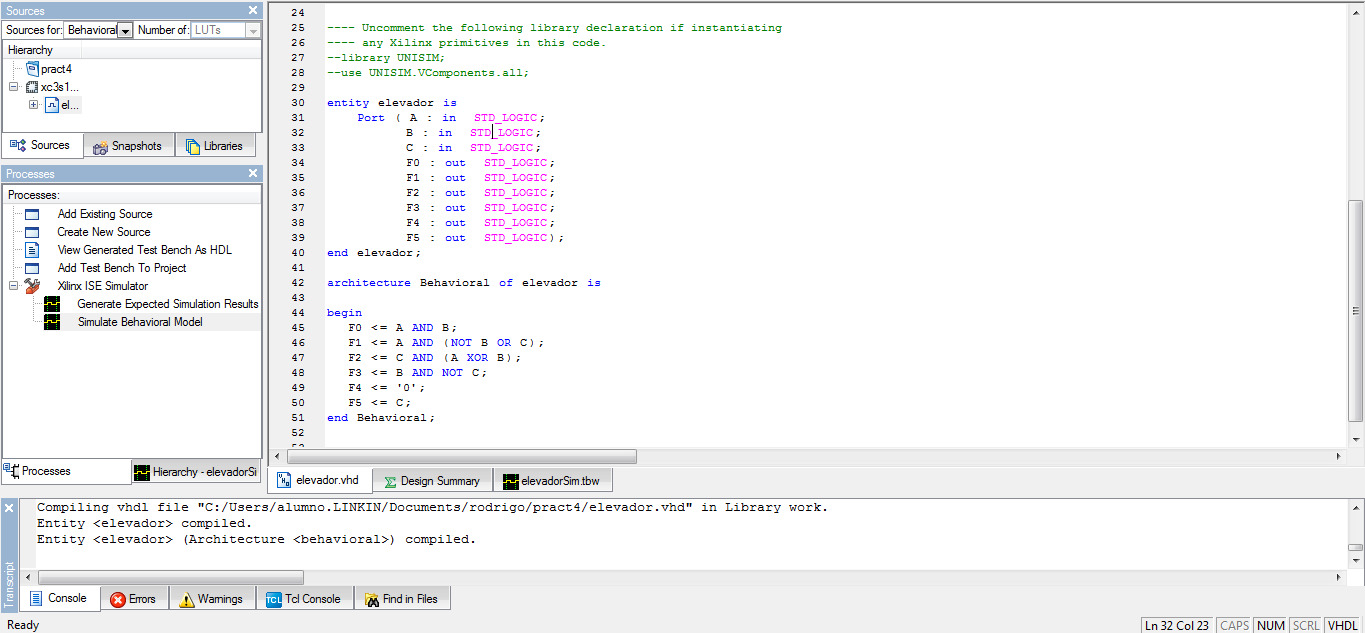
\includegraphics[width=15cm]{img/labdise_pract4/r4_img1}\\

Comprobamos que el circuito estuviera bien y para ello realizamos la simulación y probamos para diferentes valores como puede verse a continuación.\\

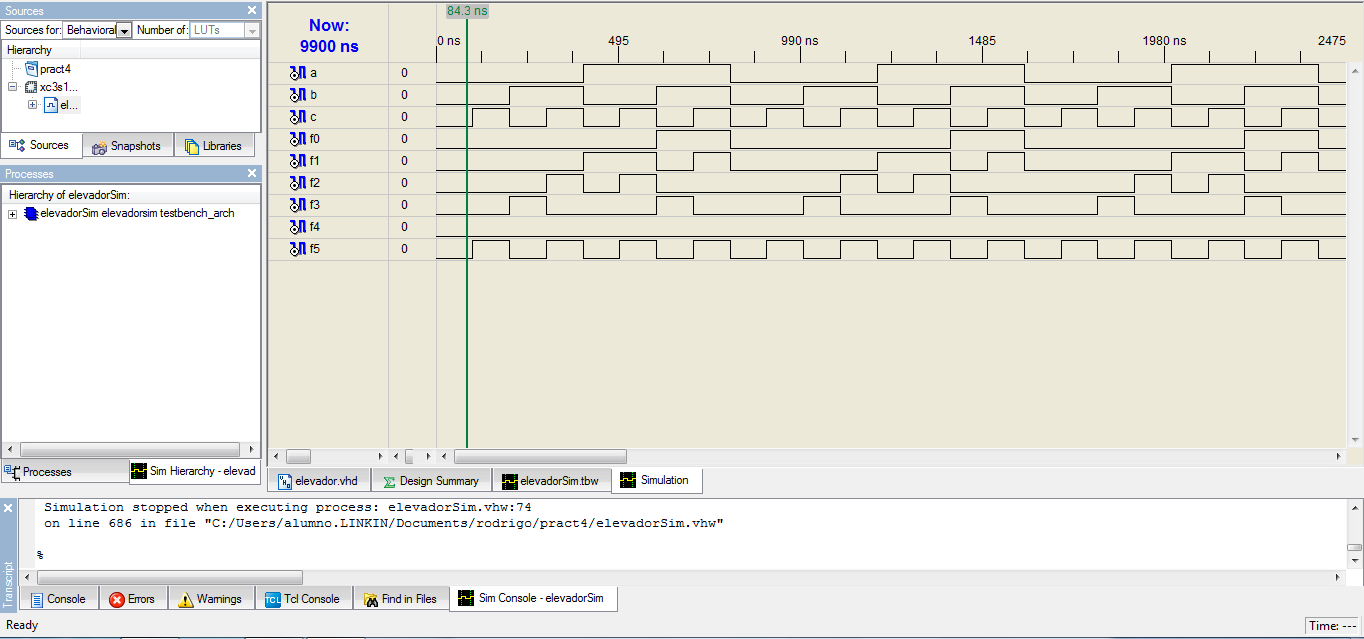
\includegraphics[width=15cm]{img/labdise_pract4/r4_img2}\\

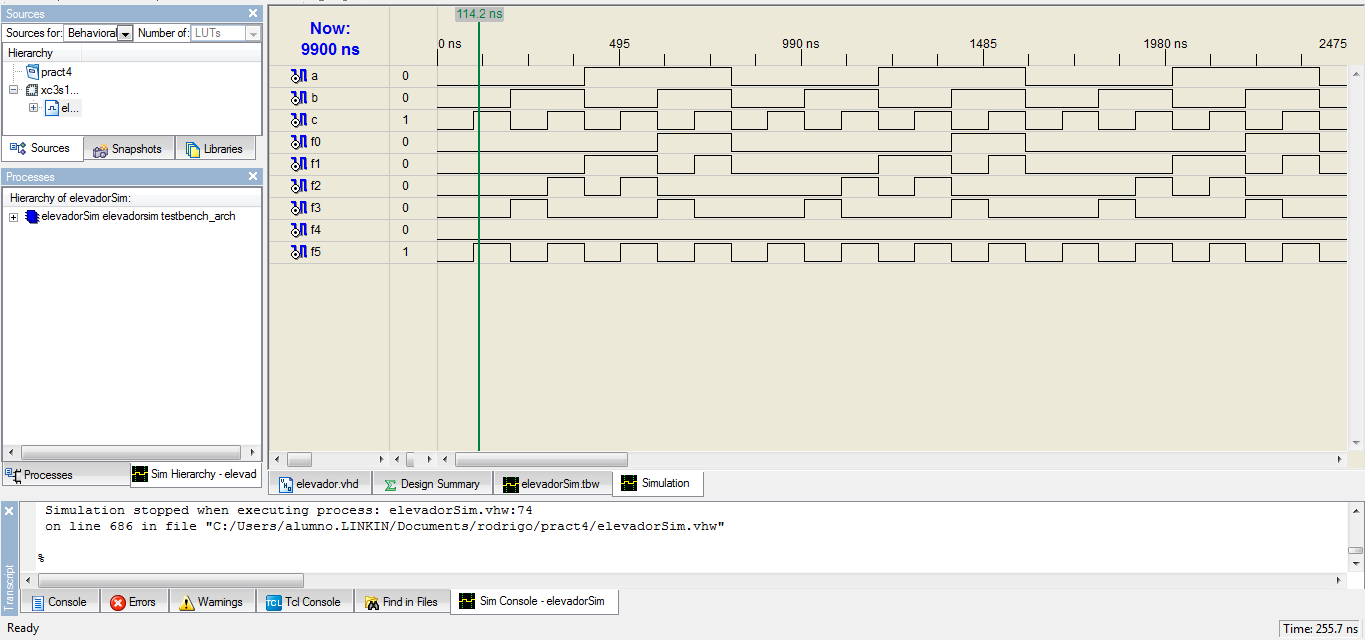
\includegraphics[width=15cm]{img/labdise_pract4/r4_img3}\\

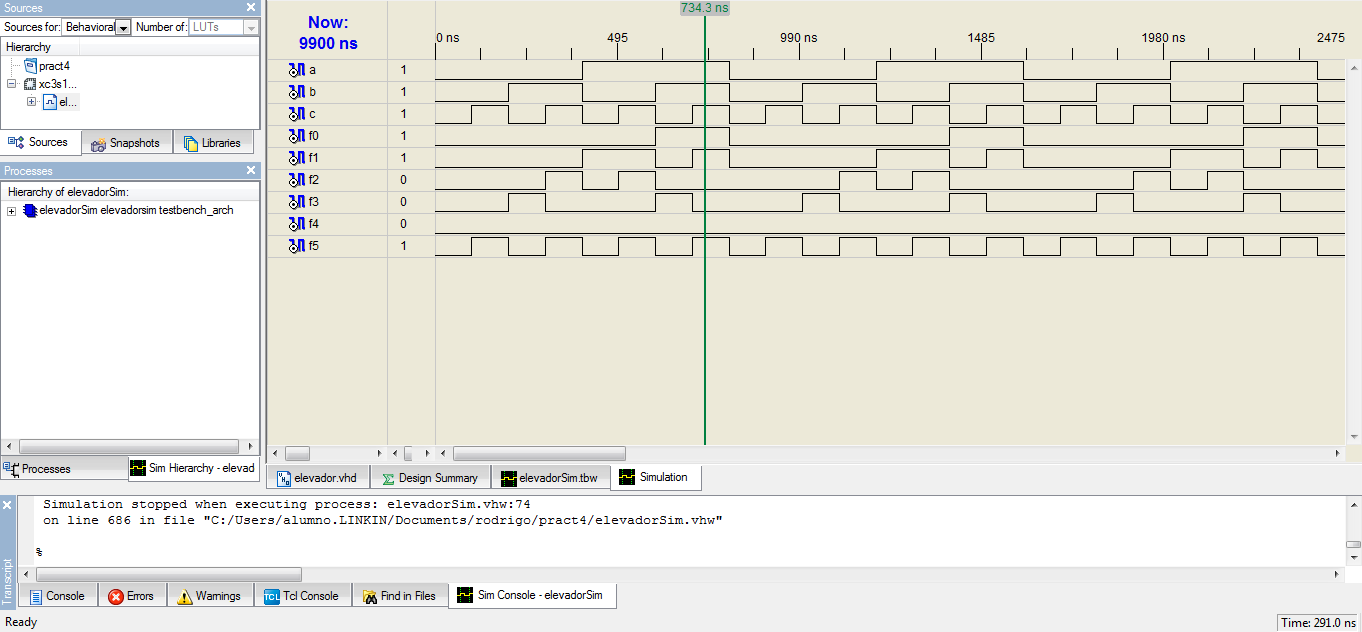
\includegraphics[width=15cm]{img/labdise_pract4/r4_img4}\\

Lorem ipsum dolor sit amet, consectetur adipiscing elit. Ut ornare neque vel nibh tempus efficitur. Nunc mollis blandit purus, posuere sagittis justo porta eget.\\

%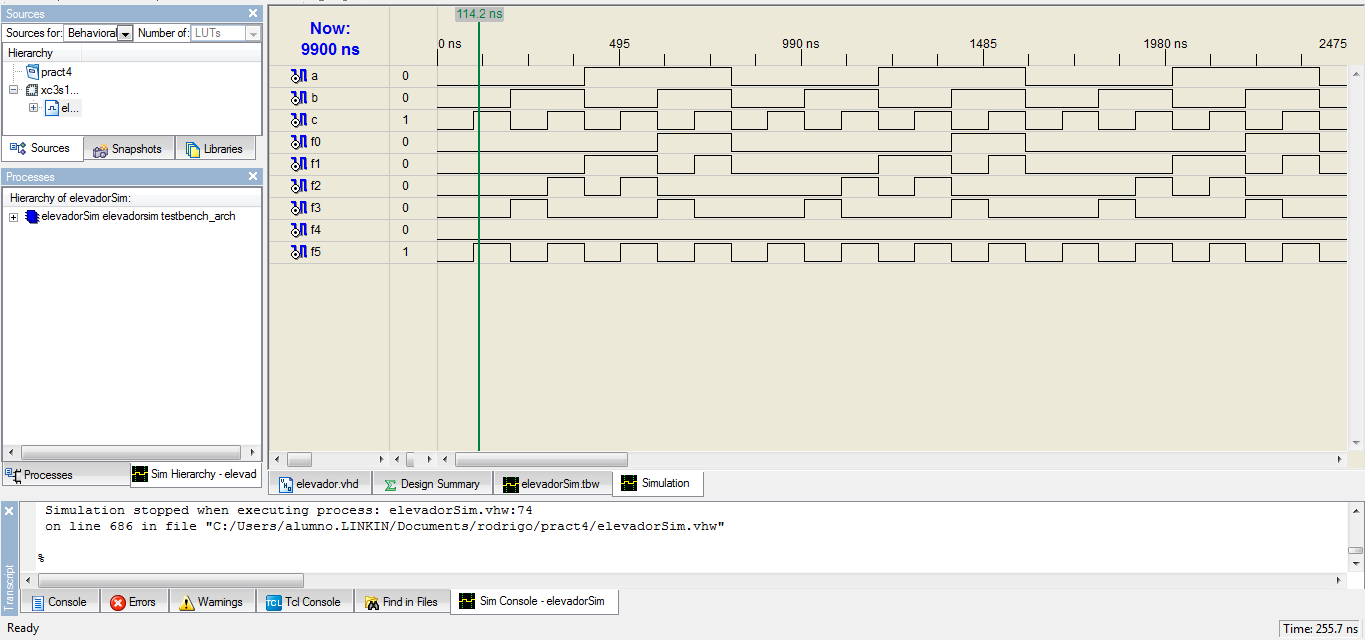
\includegraphics[width=15cm]{img/labdise_pract4/r4_img3}\\

Lorem ipsum dolor sit amet, consectetur adipiscing elit. Ut ornare neque vel nibh tempus efficitur. Nunc mollis blandit purus, posuere sagittis justo porta eget. \\

%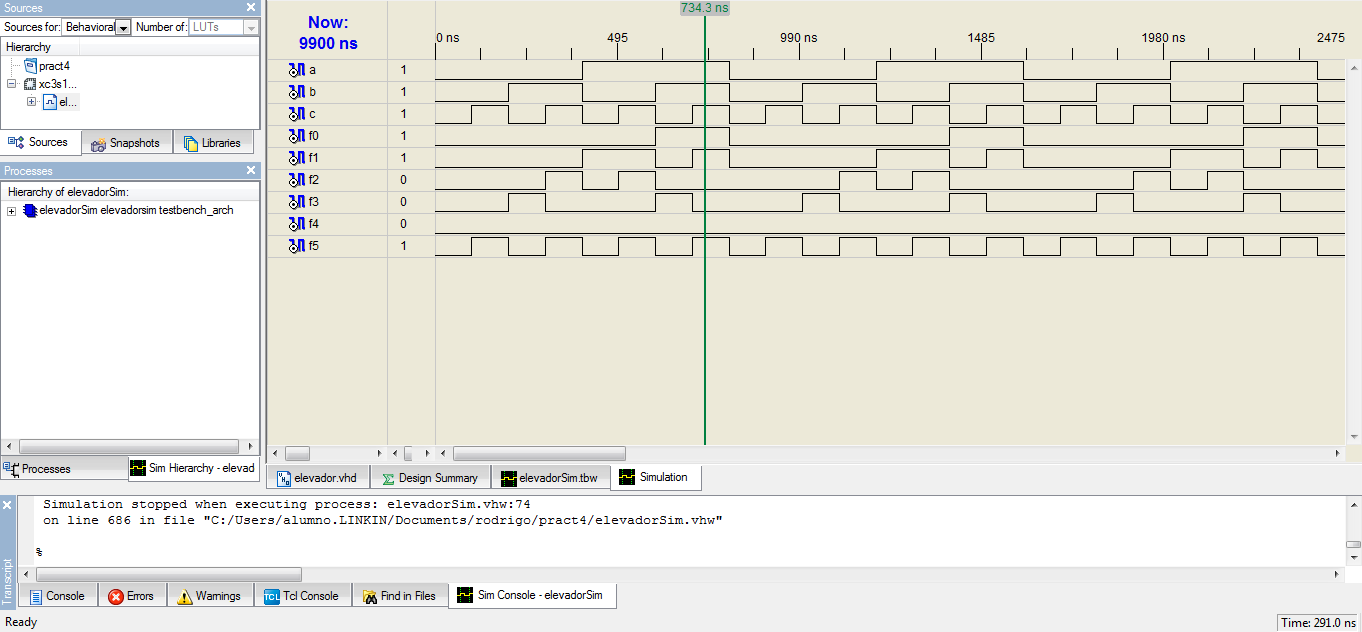
\includegraphics[width=15cm]{img/labdise_pract4/r4_img4}\\

Lorem ipsum dolor sit amet, consectetur adipiscing elit. Ut ornare neque vel nibh tempus efficitur. Nunc mollis blandit purus, posuere sagittis justo porta eget. \\

Lorem ipsum dolor sit amet, consectetur adipiscing elit. Ut ornare neque vel nibh tempus efficitur. Nunc mollis blandit purus, posuere sagittis justo porta eget..\\

%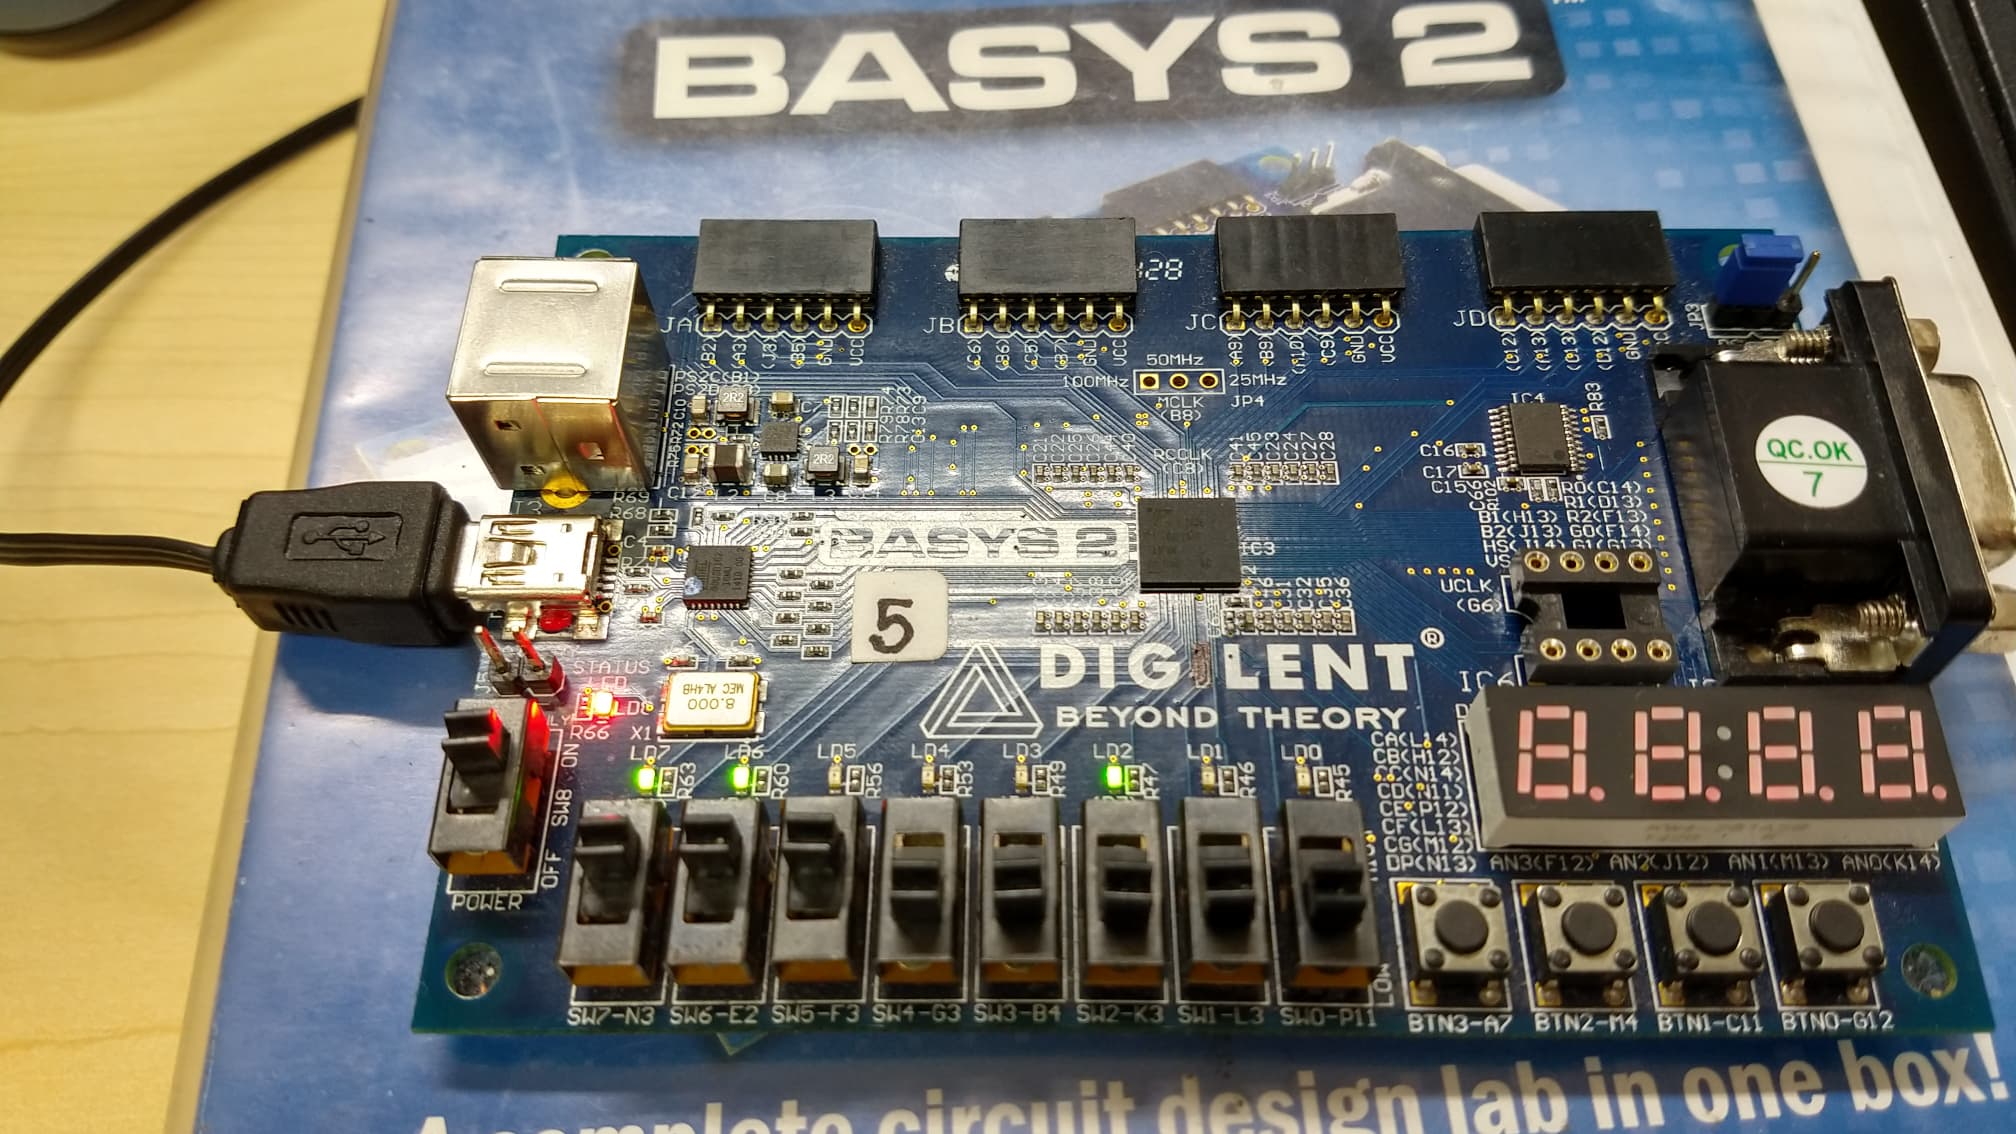
\includegraphics[width=15cm]{img/labdise_pract4/r4_img5}\\

Lorem ipsum dolor sit amet, consectetur adipiscing elit. Ut ornare neque vel nibh tempus efficitur. Nunc mollis blandit purus, posuere sagittis justo porta eget..\\

%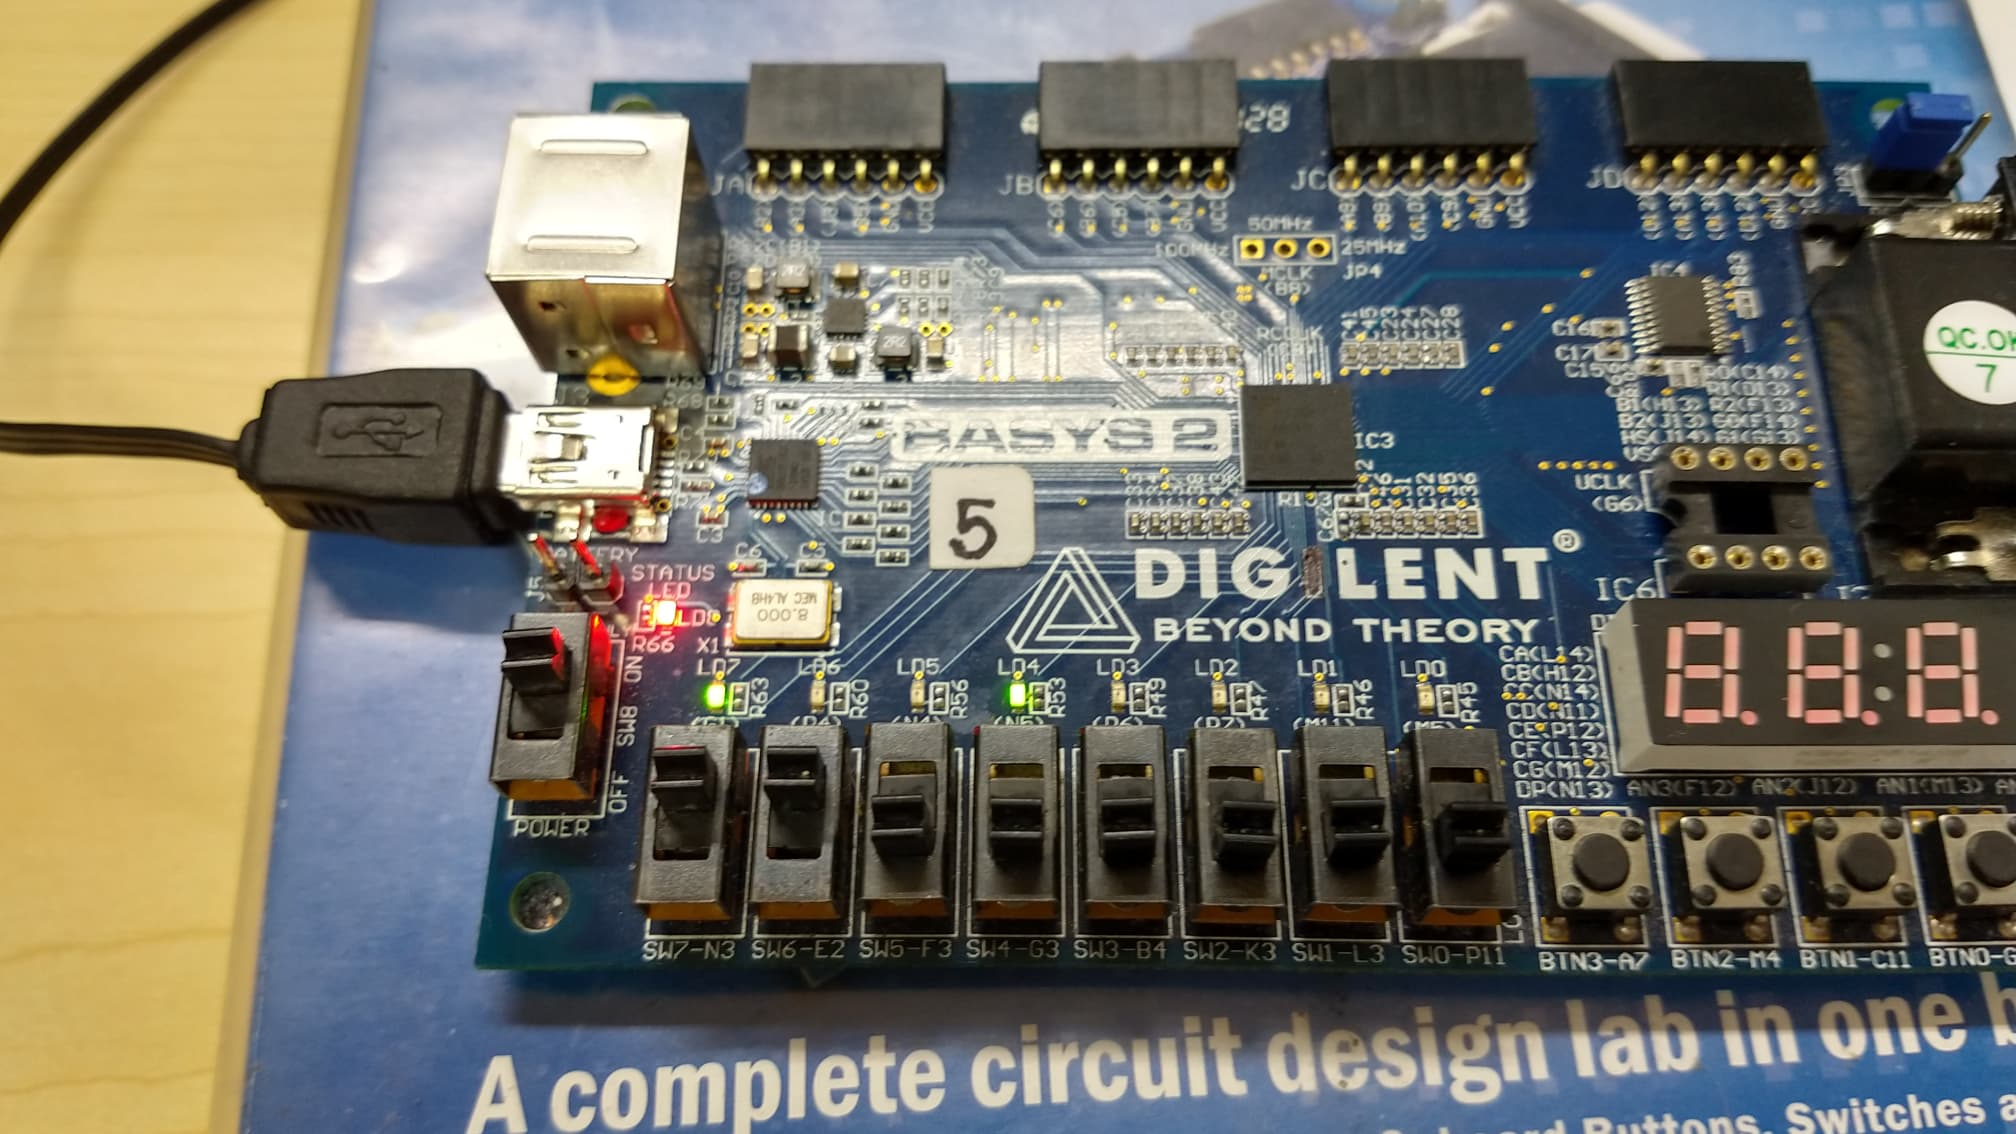
\includegraphics[width=15cm]{img/labdise_pract4/r4_img6}\\

\section{Conclusiones}

Lorem ipsum dolor sit amet, consectetur adipiscing elit. Ut ornare neque vel nibh tempus efficitur. Nunc mollis blandit purus, posuere sagittis justo porta eget.\\

Vestibulum fermentum bibendum velit, ut imperdiet elit lobortis nec. Maecenas id finibus est. Fusce sed nunc ut tellus pharetra accumsan. In venenatis quis arcu sed pretium. Donec convallis tempus vehicula. Nunc id libero vitae tortor dapibus efficitur quis at elit. Nullam eu purus egestas mauris commodo suscipit. Mauris ac turpis non nulla tempus lobortis. Pellentesque posuere vitae nisi nec vestibulum. Donec vulputate ullamcorper eros, eu mattis lorem fringilla vel. Duis at gravida leo. Sed pellentesque interdum nulla. Aenean rhoncus sagittis dignissim. Morbi viverra eleifend dolor. Aliquam finibus sem felis, non imperdiet velit laoreet sed.

\end{document}